%! Licence = CC BY-NC-SA 4.0

%! Author = gianfluetsch
%! Date = 22. Jan 2022
%! Project = icth_summary

\section{Produktmodulation}

\subsubsection{Prüfung HS2019}
Ein auf einen Träger von 20 MHz aufmoduliertes Datensignal soll mittels Produktmodulation auf eine Sendefrequenz von 100 MHz verschoben werden.\\
\begin{itemize}
    \item Mit welchen zwei Modulatorfrequenzen (Lösung 1 und 2) kann dies erreicht werden?
    \item Zeichnen Sie das zweiseitige Spektrum nach der Produktmodulation in die zwei untenstehenden Grafiken ein.
    \item Welche Filter werden in Lösung 1, respektive 2 benötigt, damit nur das Datensignal bei 100 MHz ausgesendet wird?
\end{itemize}

\begin{center}
    \vspace{-8pt}
    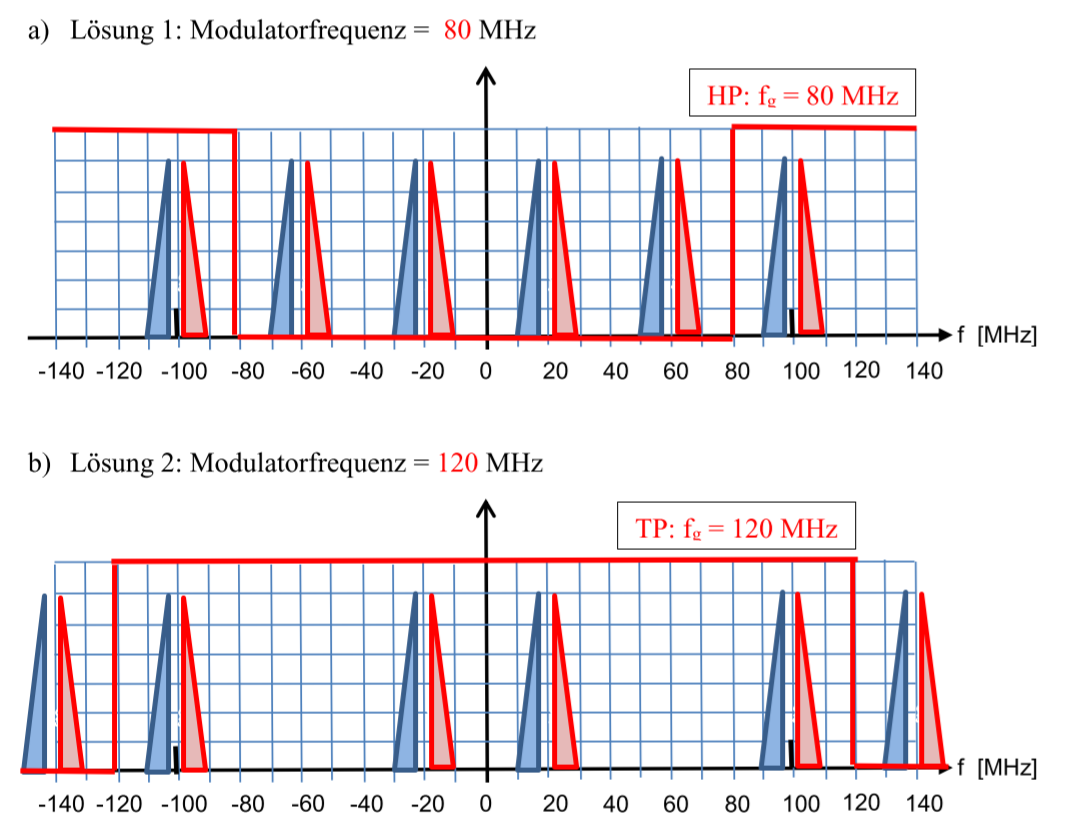
\includegraphics[width=.9\linewidth]{./10-produktmanipulation/hs2019_5}
    \vspace{-8pt}
\end{center}